\section*{Question 8}
\textit{Plot the pre-multiplied spectrum for both datasets and calculate the dominant time-scale (and hence length scale using Taylor’s hypothesis) using this data by locating the peak in this pre-mulitplied spectrum.}

\begin{figure}[!ht]
\centering
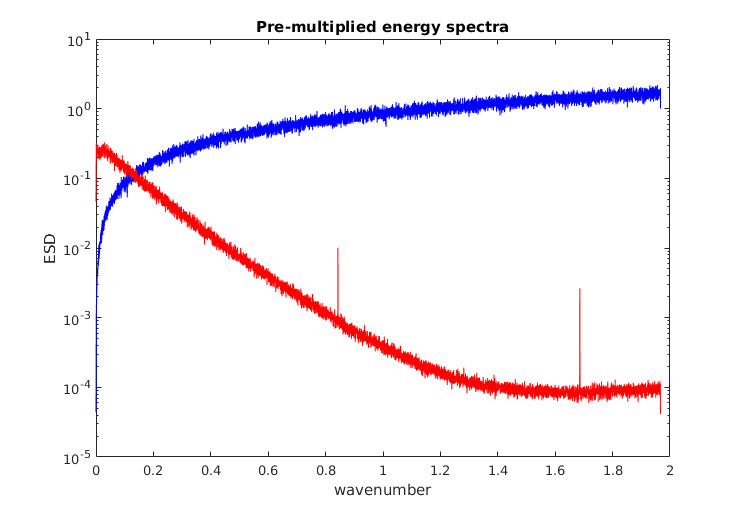
\includegraphics[scale=0.8]{./TEXT/esd-n.png}
\caption{Comparison between the energy spectral densities in the spatial domain of both flow cases as they change with wavenumber for a window size of $20'000$ data points}
\label{esd-n}
\end{figure}
